\documentclass[tikz]{standalone}

\usepackage{tikz}
\usepackage{xcolor}
\usepackage{pgfplots}
\usepackage{../tikzviolinplots}
%\usepgfplotslibrary{external}
%\tikzexternalize
\usepackage{siunitx}
\usepackage{fontspec}

\pgfplotsset{compat=1.18}
\setmainfont{Source Serif 4}[
    Renderer = OpenType,
    SizeFeatures    = {%
        {Size={-9},Font=* Caption},
        {Size={9-13},Font=*},
        {Size={14-24},Font=* Subhead},
        {Size={24-},Font=* Display}
    },
    ItalicFeatures = {%
    SizeFeatures    = {%
            {Size={-9},Font=* Caption Italic},
            {Size={9-13},Font=* Italic},
            {Size={14-24},Font=* Subhead Italic},
            {Size={24-},Font=* Display Italic}
    },
    },
    BoldFeatures = {%
    SizeFeatures    = {%
            {Size={-9},Font=* Caption Semibold},
            {Size={9-13},Font=* Semibold},
            {Size={14-24},Font=* Subhead Semibold},
            {Size={24-},Font=* Display Semibold}
    },
    },
    BoldItalicFeatures = {%
    SizeFeatures    = {%
            {Size={-9},Font=* Caption Semibold Italic},
            {Size={9-13},Font=* Semibold Italic},
            {Size={14-24},Font=* Subhead Semibold Italic},
            {Size={24-},Font=* Display Semibold Italic}
    },
    },
    Numbers         = OldStyle,
]

\usetikzlibrary{shapes,arrows,positioning,backgrounds,calc,intersections,calc,svg.path,fit,fpu}
\definecolor{ugent-re}{RGB}{220, 78, 40}        % vermilion			/ vermiljoen
\definecolor{ugent-we}{RGB}{45, 140, 168}       % no match

\begin{document}
\begin{filecontents}[overwrite]{violin-large.dat}
    A,B,C,D,E
    0.00011,0.00011,0.00011,0.00011,0.00012
    0.0001,0.0001,0.0001,0.0001,0.0001
    0.0001,0.0001,0.0001,0.0001,0.0001
    0.0001,0.0001,0.0001,0.0001,0.0001
    -0.19258,-0.07122,-0.00454,0.07875,0.03067
    -0.05095,-0.03514,-0.03145,-0.03099,-0.03138
    -0.00178,0.00963,0.02502,1.76091,0.16798
    -0.02752,-0.00622,0.00489,0.01151,0.07413
    -0.00036,0.00032,0.00026,0.0003,0.00056
    0.0001,0.0001,0.0001,0.0001,0.0001
    -0.00268,-0.00075,0.00095,0.003,0.00628
    -0.04059,-0.00228,0.0312,0.07263,0.12983
    -0.02819,-0.01031,0.00016,0.00958,0.02106
    -0.0041,-0.00256,-0.00123,0.0004,0.00317
    -0.00915,0.00166,0.01007,0.10018,0.03654
    -1.78683,-1.79078,-1.87897,-1.76577,-4.4141
    0.00019,0.00023,0.00021,0.00022,0.00041
    -0.02363,-0.01364,-0.0059,0.00238,0.02125
    -0.00046,0.00013,0.00048,0.00069,0.00104
    -3.25577,-2.04408,-2.76289,-2.48387,-8.218
    -0.00215,0.04247,0.07104,0.09231,0.07027
    -0.003,-0.00084,0.00064,0.0025,0.00279
    0.0001,0.0001,0.0001,0.0001,0.0001
    -1.78055,-1.41716,-1.19861,-1.11085,-1.12134
    0.0001,0.0001,0.0001,0.0001,0.0001
\end{filecontents}
\begin{tikzpicture}
    \pgfplotsset{height=5cm,width=6cm}
    \pgfkeys{/pgfplots/yticklabel={\addfontfeature{Numbers={Lining}}\qty[round-mode=places, round-precision=0]{\tick}{\mega{}}},}
    \violinsetoptions[
        scaled,
        averages,
    ]{
        xmin=0.3,xmax=6.2,
        ymin=-13,ymax=4,
        xlabel style={
            yshift = {-3*height("a")}
        },
        ymajorgrids=true,
        ytick distance=3,
        ylabel={№ of blocks}
    }
    \violinplot[%
        index=A,
        relative position=1,
        label={30},
        samples=100,
        average mark=*,
        average fill=black,
        average fill opacity=1.0,
        average size=1pt,
        color=ugent-we,
    ]{violin-large.dat}
    \violinplot[%
        index=B,
        relative position=2.2,
        label={60},
        samples=100,
        average mark=*,
        average fill=black,
        average fill opacity=1.0,
        average size=1pt,
        color=ugent-we,
    ]{violin-large.dat}
    \violinplot[%
        index=C,
        relative position=3.3,
        label={90},
        samples=100,
        average mark=*,
        average fill=black,
        average fill opacity=1.0,
        average size=1pt,
        color=ugent-we,
    ]{violin-large.dat}
    \violinplot[%
        index=D,
        relative position=4.4,
        label={120},
        samples=100,
        average mark=*,
        average fill=black,
        average fill opacity=1.0,
        average size=1pt,
        color=ugent-we,
    ]{violin-large.dat}
    %! parser = off
    \pgfkeys{
        /pgfplots/xlabel={Execution models (\textsc{em-})},
    };
    %! parser = on
    \violinplot[%
        index=E,
        relative position=5.5,
        samples=100,
        label={asap},
        average mark=*,
        average fill=black,
        average fill opacity=1.0,
        average size=1pt,
    ]{violin-large.dat}
\end{tikzpicture}
\end{document}
